%%%%%%%%%%%%%%%%%%%%%%%%%%%%%%%%%%%%%%%%%
% University Assignment Title Page 
% LaTeX Template
% Version 1.0 (27/12/12)
%
% This template has been downloaded from:
% http://www.LaTeXTemplates.com
%
% Original author:
% WikiBooks (http://en.wikibooks.org/wiki/LaTeX/Title_Creation)
%
% License:
% CC BY-NC-SA 3.0 (http://creativecommons.org/licenses/by-nc-sa/3.0/)
%
%%%%%%%%%%%%%%%%%%%%%%%%%%%%%%%%%%%%%%%%%
%\title{Title page with logo}
%----------------------------------------------------------------------------------------
%	PACKAGES AND OTHER DOCUMENT CONFIGURATIONS
%----------------------------------------------------------------------------------------

\documentclass[12pt]{article}
\usepackage[english]{babel}
\usepackage[utf8]{inputenc}
\usepackage{natbib}
\usepackage{amsmath}
\usepackage{color}
\usepackage[explicit]{titlesec}
\usepackage[hyphens,spaces,obeyspaces]{url}
\usepackage{graphicx}
\usepackage{caption}
\usepackage{subcaption}
\usepackage{grffile}
\usepackage{listings}

\lstset{language=python,keywordstyle={\bfseries \color{blue}}}
\usepackage{booktabs}

\begin{document}

\begin{titlepage}

\newcommand{\HRule}{\rule{\linewidth}{0.5mm}} % Defines a new command for the horizontal lines, change thickness here

\center % Center everything on the page
 
%----------------------------------------------------------------------------------------
%	HEADING SECTIONS
%----------------------------------------------------------------------------------------

\textsc{\LARGE University of St Andrews}\\[1.5cm] % Name of your university/college
\textsc{\Large Machine Learning}\\[0.5cm] % Major heading such as course name
\textsc{\large CS5014}\\[0.5cm] % Minor heading such as course title

%----------------------------------------------------------------------------------------
%	TITLE SECTION
%----------------------------------------------------------------------------------------

\HRule \\[0.4cm]
{ \huge \bfseries Classification}\\[0.4cm] % Title of your document
\HRule \\[1.5cm]
 
%----------------------------------------------------------------------------------------
%	AUTHOR SECTION
%----------------------------------------------------------------------------------------


\Large \emph{Author:}\\
 \textsc{150008022}\\[1cm] % Your name
 
%----------------------------------------------------------------------------------------
%	DATE SECTION
%----------------------------------------------------------------------------------------

{\large \today}\\[2cm] % Date, change the \today to a set date if you want to be precise

%----------------------------------------------------------------------------------------
%	LOGO SECTION
%---------------------------------------------------------------------------------------


\includegraphics[width = 4cm]{images/standrewslogo.png}
 
%----------------------------------------------------------------------------------------

\vfill % Fill the rest of the page with whitespace

\end{titlepage}

\subsection*{Goal}

The goal of this practical is to analyse a dataset in order to produce a classification model that can make predictions based on a set of inputs.

\tableofcontents

\pagebreak
\pagenumbering{arabic}
\setcounter{page}{1} 

\section{Loading Data}

To load the data, the paths to the relevant files are supplied as arguments to the \emph{\_\_main\_\_.py} script. The \emph{pandas} module was used to load the file contents into \emph{DataFrames}.

A test set was isolated from the original data using an 80\%-20\% split. Stratification was used to ensure that all classes were represented in the training data. Since the dataset was originally grouped by output class, the order of the samples were shuffled. This would avoid the later model being trained on several similiar instances in a row, which can have an affect on some algorithms performance.

\section{Cleaning Data}

When originally loading the CSV files the parameter to raise an exception on missing or extra columns was included, and so it could be assumed that all rows had the same number of columns. The \lstinline{dtype=float} argument was also passed when loading the data to ensure that each column contained the expected numerical data. Any rows containing empty or \lstinline{NaN} values were dropped from the dataset.

\section{Data Visualisation and Analysis}

The input CSV was understood to have the structure shown in figure \ref{fig:structure}. Each value is either the mean, minimum, or maximum reading from 100 radar pulses for a single component of a channel. Each channel is comprised of 256 components.

\begin{figure}[!ht]
	\centering
	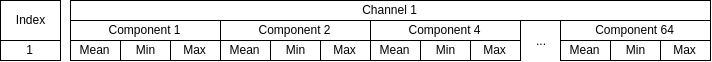
\includegraphics[width=\linewidth]{images/structure}
	\caption{The structure of each row of the CSV file which is repeated for minimum and maximum values.}
	\label{fig:structure}
\end{figure}

The mean, min, and max values were plotted for each channel for each sensor. The plots of the means of each channel for the book and plastic case objects are shown in figures \ref{fig:book} and \ref{fig:plasticcase} respectively. The difference between the resulting signals from the two objects are very clear.

\begin{figure}[!ht]
	\centering
	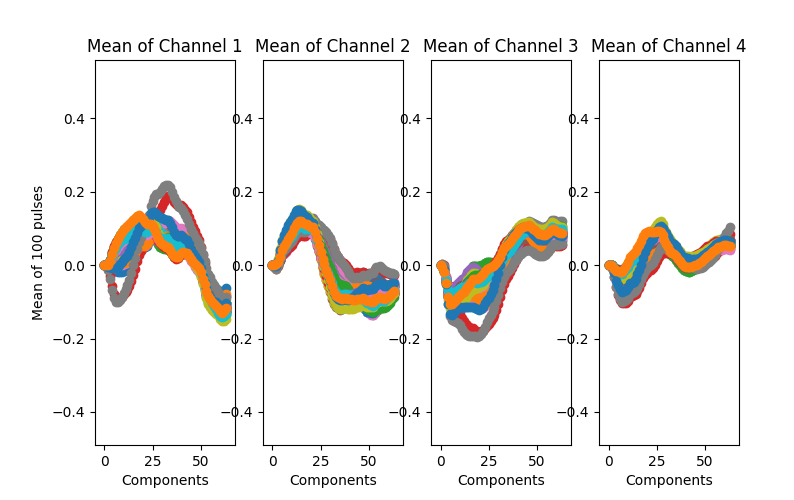
\includegraphics[width=\linewidth]{images/book}
	\caption{Mean of each channel measured for the book}
	\label{fig:book}
\end{figure}

\begin{figure}[!ht]
	\centering
	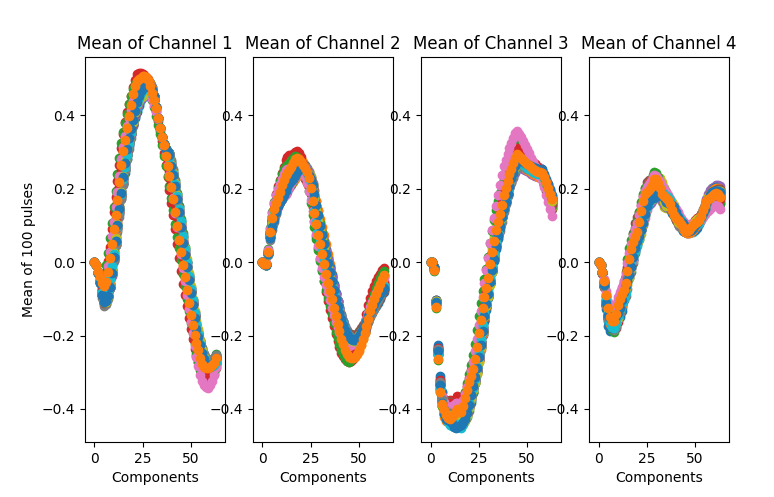
\includegraphics[width=\linewidth]{images/plasticcase}
	\caption{Mean of each channel measured for the plastic case}
	\label{fig:plasticcase}
\end{figure}

In the binary dataset, the minimum and maximum components observed all followed a similiar shape as the average, but the book class did contain one severe outlier in two plots. The full plots are included in the submission under \url{plots/binarybook.png} and \url{plots/binaryplasticcase}, in which the plot of the minimum components in channel one and the maximum components in channel three both include one row of outliers. 
Since the average did not deviate from other components for that class, it seemed fair to say that these maximum and minimum readings were outliers. Instead of removing them and risking producing a biased model, the row was left in the data set. A real world application of the sensor would likely involve noise, and so it made sense to train the model to be able to cope with anomalies. The existence of these outliers was however noted when choosing a cost function however in order to try and minimise their affect.

The same plots were made for the multiclass dataset, and from this it was clear that each material produced very different results, with varying levels of consistency. For example, the data aquired when the radar sensor was applied to a human hand varied wildly, whilst the readings for the plastic cover were a very clear sinusoidal shape. These plots can be found in \url{plots/multiclass*}.

Since the radar signature was determined by the reflection of the radar pulses on the surface and interior structure of each object, the resulting plots were understandable. For example, the plastic case shows a very consistent pattern likely due to the fact that it is composed of a single material in a uniform structure, whilst the human hand produces a very chaotic signature since it is composed of many different materials, especially fluids in motion.

\begin{figure}
\centering
\begin{subfigure}{.5\textwidth}
  \centering
  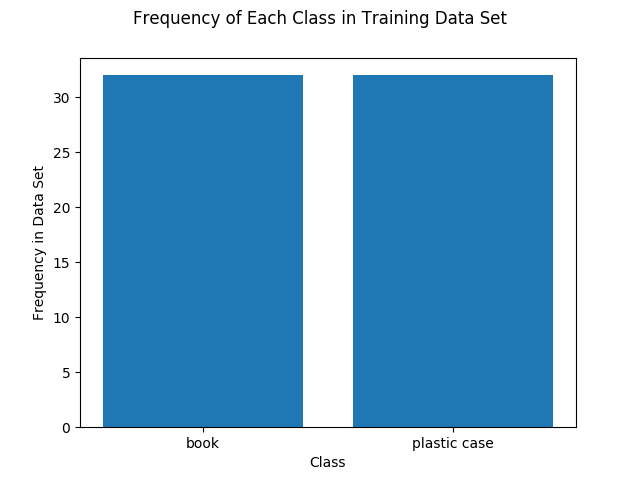
\includegraphics[width=\linewidth]{images/binaryfrequencies}
  \caption{Binary}
  \label{fig:sub1}
\end{subfigure}%
\begin{subfigure}{.5\textwidth}
  \centering
  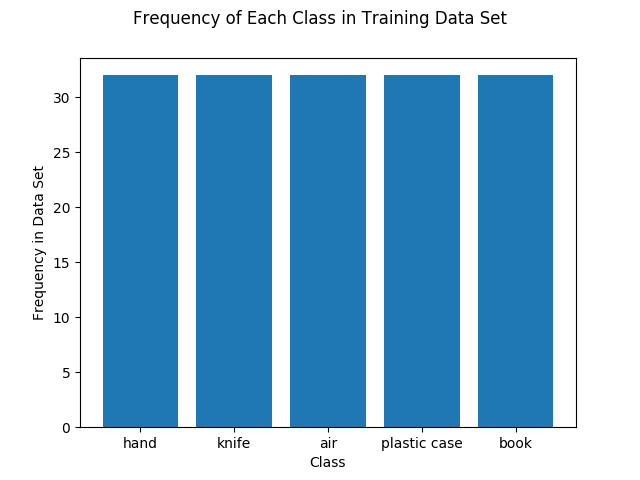
\includegraphics[width=\linewidth]{images/multiclassfrequencies}
  \caption{Multiclass}
  \label{fig:sub2}
\end{subfigure}
\caption{Frequencies of each class in the binary and multiclass training data sets}
\label{fig:classdist}
\end{figure}

The training data set was shown not be skewed by plotting the distribution of each class (figure\ref{fig:classdist}). The equal distribution of each class meant that cross validation of a classifier that always guesses the same class will have a ratio of correct predictions inversely proportional to number of classes in the training data set. 

All data from the feature set had values between -1 and 1, and from the plots of all classes it was noticed that the different classes had different global minumum and maximums for each channel. For example, the components of samples for air did not surpass 0.1, 0.25 for books, 0.5 for plastic case, and 0.75 to 1 for hand and knife. Based on this and the fact that there were no outliers and the values were evenly distributed, normalisation was used over standardisation. Plotting the normalised data and comparing it to the plots of the original data reinforced this decision, as the shape and scale of the resulting plots had been maintained.

\section{Feature Selection}

The large number of features available in the dataset makes computation of any model more expensive. In order to have an effective classifier, there should be at least five examples of each combination of values from each feature in the training data \cite{mincombs}, which our dataset is unable to provide. Therefore a reduction of the feature set was considered necessary.

The visualisations of the training data showed that each class had very different levels of variation between each sample, and this variation could be used to identify a class. However our model would need to identify the class based on a single sample, and so this variation could not be relied on. 

It was observed that the plots of each channel for the mean, minumum, and average were very similiar for each sample within a class. For this reason, all components were dropped except those based on the average of 100 pulses. 

Principal component analysis (PCA) was then used to further reduce the number of features. PCA works by projecting the data onto the hyperplane that retains the most of the original variance in the dataset. By producing vectors that map and combine the original features to another set, PCA concentrates as much information into the first principle component, and then as much of whatever remains into the second component, and so on. Since the mapping combines features, the resulting components do not have any real meaning, though the original data can be recovered from the resulting principal components.

Initially, to try and understand PCA a plot of the first two principals components was produced (Figure \ref{fig:pca1}. The first two principal components alone accounted for 82\% of the original variance.

\begin{figure}[!ht]
	\centering
	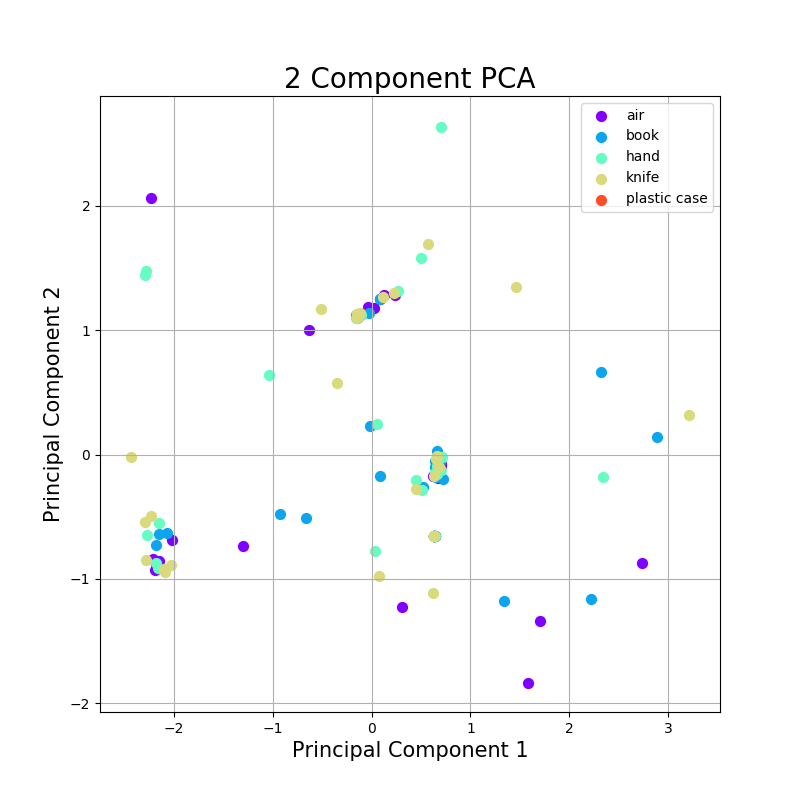
\includegraphics[width=0.8\linewidth]{images/2dpca}
	\caption{The first two principal components, coloured according to their class.}
	\label{fig:pca1}
\end{figure}

To show how variance changes as the number of principal components increases, the explained variance ratios were also plotted against the number of dimensions in figure \ref{fig:explainedvariance}. The return on increasing dimensions becomes miniscule after 20 dimensions.
For the actual model, the PCA was configured to select the number of components that would retain 95\% of the original variance. This reduced the feature set from 256 to 6.

\begin{figure}[!ht]
	\centering
	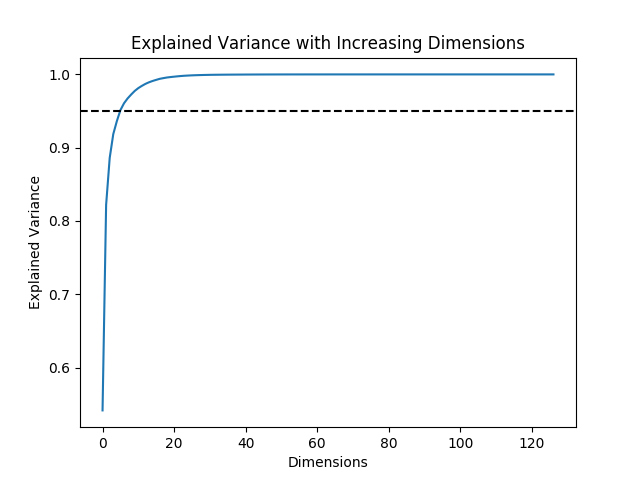
\includegraphics[width=0.8\linewidth]{images/explainedvariance}
	\caption{The elbow curve of explained variance that results from increasing the number of dimensions. The dashed line is drawn at our models chosen variance.}
	\label{fig:explainedvariance}
\end{figure}

The PCA used method requires loading the entire dataset into memory. Alternative methods exists such as incremental PCA and random PCA that can be used for online and batched learning.

\section{Model Selection and Training}

\begin{figure}[!ht]
	\centering
	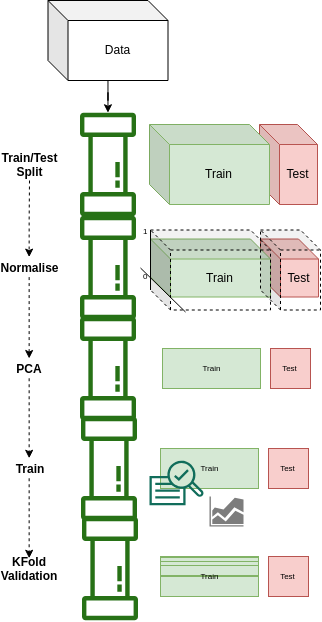
\includegraphics[width=0.5\linewidth]{images/pipe}
	\caption{The pipeline used by the submission.}
	\label{fig:pipeline}
\end{figure}

Multiclass classifcation can be implemented using binary classifiers through two methods, one-vs-one and one-vs-all. One-vs-all involves training an individual classifier per class, and each classifier is only able to state if the input represents its class or not. Since the training data used has an equal distribution of each class, each classifier would be trained on skewed data with far more negatives than positives as demonstrated in figure \ref{fig:classifierperclass}. This method would require as many classifiers as there are classes \cite{handson}.

\begin{figure}[!ht]
	\centering
	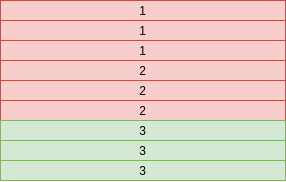
\includegraphics[width=0.5\linewidth]{images/classifierperclass}
	\caption{Distribution of negative and positive samples for a classifier trained to identify either class '3' or 'not 3' when each class is equally represented}
	\label{fig:classifierperclass}
\end{figure}

A one-vs-one classifier requires a classifier exists for each pair of classes. Each classifier will predict a value from the two classes it was trained to identify, and the resulting prediction will be the class that was chosen by the most classifiers. This method requires $n (n - 1)^2$ classifiers, where n is the number of classes.

There also exist dedicated multiclass classifiers with different advantages and implementations.

Since the RadarCat \cite{radarcat} technology is intended to be able to allow users to identify and catalogue various every day objects, both the one-vs-one and one-vs-all approaches would involve a large number of classifiers being trained. Therefore an approach that required fewer classifiers would probably be preferred. 

On the other hand, the Soli \cite{soli} technology used by RadarCat was designed with the intention of recognising hand gestures, and so being able to generalise well when trained on fewer classes would likely be favoured in that case (i.e. handling many variations of the same hand gesture).

Another possible solution that could reduce the number of classifiers needed as the number of classes grow is to create a hierarchy of classifiers. Each node has an "is-a" relationship with its parent in the tree, and prediction involves starting with a very generic classifier, and gradually getting more specific. \cite{heirarchy} for example used such classifier to identify the musical genre of an audio clip using a heirachical structure. Though it performed similiarly to a flat classifier approach, it would be easier to include new classes. This would be useful for the RadarCat use case as the number of objects it is used to identify grows.

The ability to provide online learning (or at least batch learning) would also be useful, as user feedback could provide a method for crowdsourcing samples for further supervised learning. Crowdsourced data collection for producing data for supervised learning has famously been applied by projects such as reCAPTCHA \cite{captcha}, and a similiar method could be used by RadarCat to improve its error rate.

With the previous information in mind (and for the sake of evaluation and comparison), an inherently multiclass method (Random Forest) and a one-vs-one method (Stochastic Gradient Descent) were chosen for the first and second models respectively. 

\subsection{Random Forest Classifier}

The random forest classifier was chosen due to its robustness when dealing with noisy data, which would definitely be present in real world applications \cite{rf}. The number of classifiers would not grow with the number of classes, though training would be slower. Especially so in this case due to the high number of dimensions involved.

Random forests work by building a collection of decision trees which each have their own set of rules to narrow down the class and make a prediction. Instead of exclusively using a single decision tree for classifying, the random forest will take an average of all its decision trees to make its decision. Increasing the number of trees used can make predictions more stable, but will require more memory and computation. 

An rough starting point for finding the best hyperparameters for the random forest classifier was discovered by using a randomised search following the process described by \cite{search}. Then the best hyperparameters were found by using a grid search. If grid search suggested that the best parameter was at the limit of a given range (for example, best max depth was ten, and the lowest depth in the search was ten) , the search was repeated with the range of values lowered/increased in case the best value was actually less than what the search yielded. 
This process was carried out for both the multiclass and binary datasets, as it was suspected that the multiclass random forest classifier would require a larger number of estimators (the number of trees). This turned out to be true, and the resulting hyperparameters that were different between binary and multiclass searches are shown in table \ref{tbl:hyper}. The best parameters for the multiclass model were chosen for the end model, since only two models were to be submitted and using two sets of hyperparameters would effectively produce two different models.

\begin{table}[!h]
\centering
\begin{tabular}{@{}l|rr@{}}
\toprule
Parameter            & Binary & Multiclass \\ \midrule
Max Depth            & 2      & 4          \\
Number of Estimators & 50     & 700       
\end{tabular}
\caption{Hyperparameters for random forest that were different when fitted on binary and multiclass data sets.}
\label{tbl:hyper}
\end{table}

The benefits of the hyper parameter tuning can be seen in figure \ref{fig:beforeandafterrf}. Whilst the model still has some trouble telling the difference between the hand and knife signals, it no longer incorrectly identifies the hand signal as a book or as air.

\begin{figure}[!ht]
\centering
\begin{subfigure}{.5\textwidth}
  \centering
  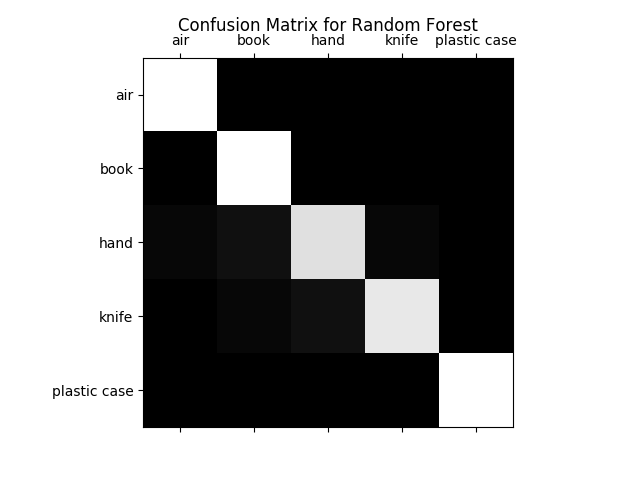
\includegraphics[width=\linewidth]{images/beforerf}
	\caption{Before}
  \label{fig:beforerf}
\end{subfigure}%
\begin{subfigure}{.5\textwidth}
  \centering
  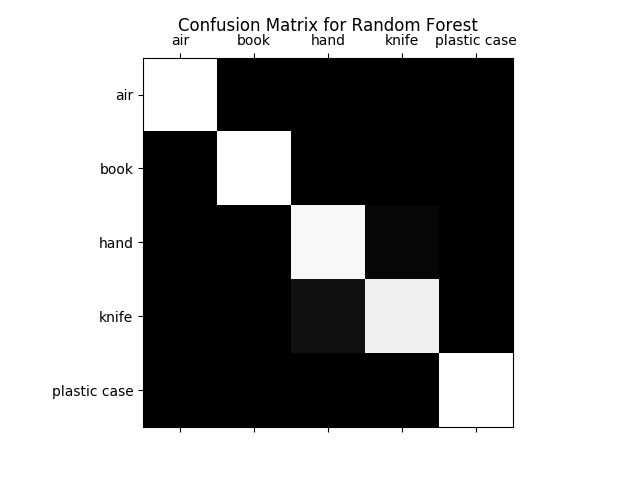
\includegraphics[width=\linewidth]{images/afterrf}
  \caption{After}
  \label{fig:afterrf}
\end{subfigure}
\caption{Confusion matrices produced by 10-fold cross validation before and after hyperparameter tuning.}
\label{fig:beforeandafterrf}
\end{figure}

\subsection{Stochastic Gradient Descent Classifier}

One-vs-one was implemented using the Stochastic Gradient Descent Classifier (SGDClassifier). It supports online and batch learning and it considers one point at a time rather than the entire dataset when learning. For the binary dataset, one-vs-one would simply reduce to a single classifier, and for the multiclass model it would require a classifier for each pair of classes.

SGD generally works by selecting a random sample at each step, and computing the gradient using that sample in order to minimize a cost function. Due to this randomness, SGD does not suffer from the local minimum problem to the same degree as batch gradient descent. The learning rate determines how quickly the step size decreases, and can determine how close to the minimum the algorithm can get. \cite{sgd} describe SGD as having two phases: a drift phase and a diffusion phase. The former is where the algorithm explores a large portion of the solution space, then as it converges upon a minimum it enters the far more chaotic diffusion phase. 

The SGDs learning rate is one of the available parameters that can determine its performance. The best value was determined using the same random search then grid search that was used for the previous model.
The hinge loss function was chosen over logistic loss due to being less sensitive to outliers. The SGDClassifier also includes a penalty parameter which penalises higher degree polynomials which generally are a sign of overfitting in the model. This way simpler models are favoured over complex models, and complexity is only introduced if it reduces the error sufficiently. This process is called regularisation.

The two regularisers considered were ridge (L2) and lasso (L1) regression. L1 can reduce the contribution of less important features to zero in the model, which can produce sparse models, whilst L2 reduces all coefficients by the same factor which will not eliminate any features. L2 was chosen by comparing the performance of the model using both.

\begin{figure}[!ht]
\centering
\begin{subfigure}{.5\textwidth}
  \centering
  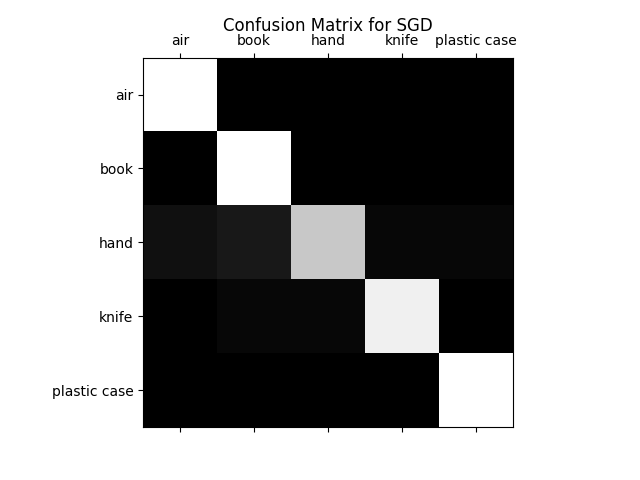
\includegraphics[width=\linewidth]{images/beforesgd}
	\caption{Before}
  \label{fig:beforesgd}
\end{subfigure}%
\begin{subfigure}{.5\textwidth}
  \centering
  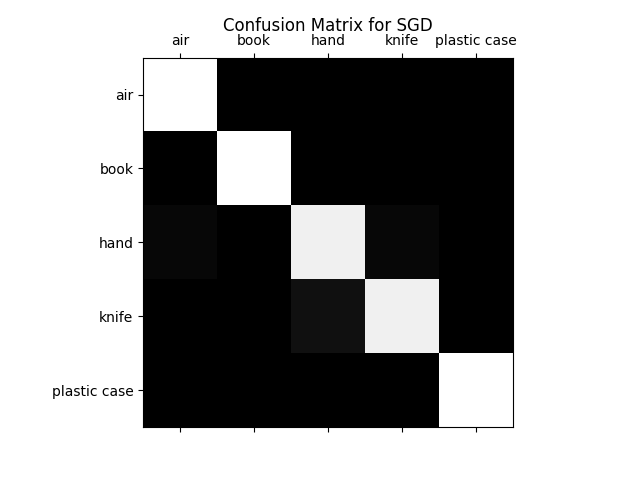
\includegraphics[width=\linewidth]{images/aftersgd}
  \caption{After}
  \label{fig:aftersgd}
\end{subfigure}
\caption{Confusion matrices produced by 10-fold cross validation before and after hyperparameter tuning.}
\label{fig:beforeandaftersgd}
\end{figure}

The model suffered from the same confusion between hand and knife samples, but would also missclassify hand as air unlike the random forest classifier. 

\section{Evaluation and Comparison}

Finally, with both models trained, tuned, and evaluated, they were then applied to the test data set.

\subsection{Binary}

Figure \ref{fig:testbinary} shows the resulting confusion matrix produced by the model when applied to the binary test data. It appears to be very effective in predicting the difference between book and plastic case.

\begin{figure}[!ht]
\centering
\begin{subfigure}{.5\textwidth}
  \centering
  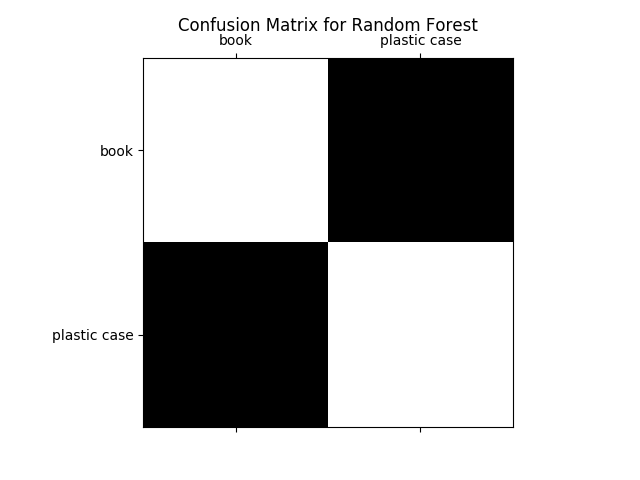
\includegraphics[width=\linewidth]{images/btestrf}
	\caption{Random Forest}
  \label{fig:brf}
\end{subfigure}%
\begin{subfigure}{.5\textwidth}
  \centering
  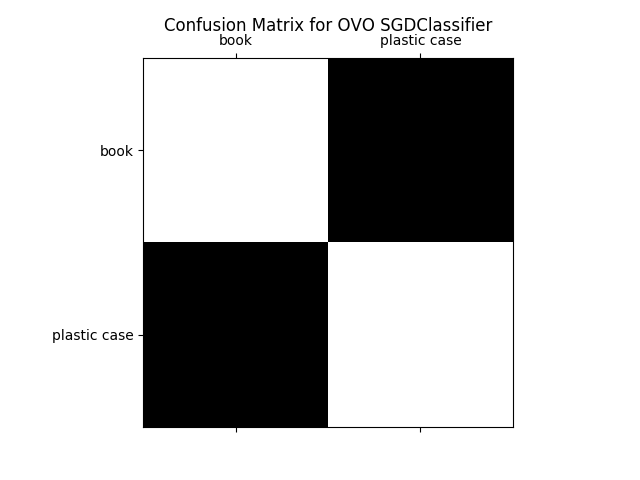
\includegraphics[width=\linewidth]{images/btestsgd}
  \caption{SGD}
  \label{fig:bsgd}
\end{subfigure}
\caption{Confusion matrices produced by the models applied to the binary test data.}
\label{fig:testbinary}
\end{figure}

\subsection{Multiclass}

Figure \ref{fig:testmulticlass} shows the resulting confusion matrix produced by the model when applied to the multiclass test data. The test data shows better performance for both models when compared to the earlier k-fold cross validation evalations on the training data. This suggests that the models have not been overfitted. 

\begin{figure}[!ht]
\centering
\begin{subfigure}{.5\textwidth}
  \centering
  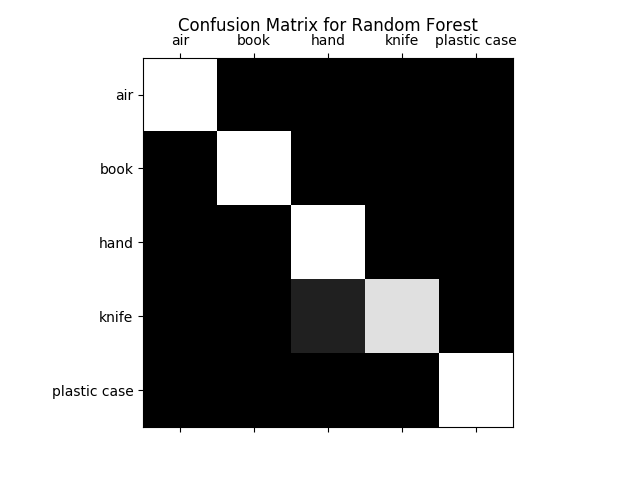
\includegraphics[width=\linewidth]{images/mctestrf}
	\caption{Random Forest}
  \label{fig:mcrf}
\end{subfigure}%
\begin{subfigure}{.5\textwidth}
  \centering
  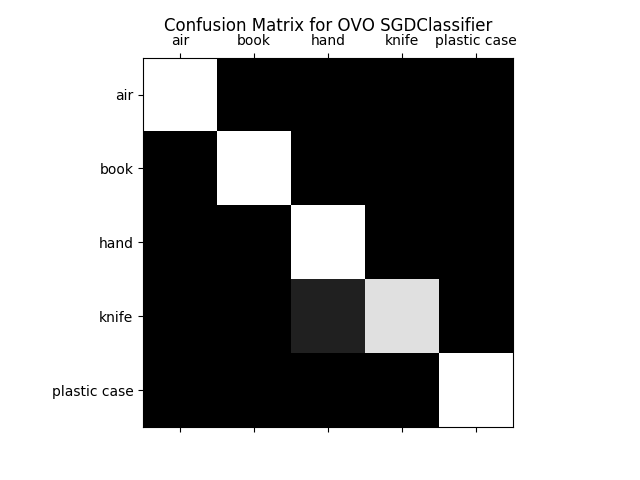
\includegraphics[width=\linewidth]{images/mctestsgd}
  \caption{OvO SGD}
  \label{fig:mcsgd}
\end{subfigure}
\caption{Confusion matrices produced by the models applied to the binary test data.}
\label{fig:testmulticlass}
\end{figure}

\section{Discussion}

Both seem to perform equally well, and both seem to missclassify knife as hand for some inputs. No synthetic features were produced during feature extraction mostly due to a lack of knowledge of exactly how the data was acquired and what it represented, but it is likely that finding other features that characterise the signals in the samples could reduce this missclassification.

Due to the similiar performance of the two models, it was difficult to choose one to classify the unlabeled test data given. However, the SGD classifier performed less well during k-fold validation and so the random forest classifier was chosen.

A lot of the time spent on this submission was focused on understanding PCA and the data that was being worked with. Given more time, I would have like to produce more synthetic features. The signals were visually different as shown in the visualisation section, and so it is likely that there is a way of mathemtically defining this difference in such a way that can be used as a feature. PCA was used in the hopes that it would be able to identify which components were the most useful for identifying each signal, but due to the abstract nature of the features it produces it is difficult to understand if this was achieved. 

\bibliographystyle{unsrt}
\bibliography{mybib}

\end{document}
